\chapter{Summary and Conclusions}
\label{cp.conc}

Over the previous century, astronomers have moved from manual observations to automated observatories, from solitary labs to worldwide collaborations, and from catalogs containing tens of thousands of stars to those containing millions. 
It is, therefore, not surprising that scholars have begun to experiment with data-driven and computationally intensive analysis methods. 
This dissertation demonstrates using one of these methods, namely Bayesian inference. 
This dissertation presents the application of Bayesian inference to estimate the significance of gravitational-wave candidates with intermediate-mass black holes. 
Even though no IMBHs were discovered, the approach supports the existence of eight stellar-mass binary black holes not previously reported in the first gravitational-wave transient catalog, GWTC-1~\cite{bcr_imbh_search}. 
In addition, the thesis demonstrates a novel use of Bayesian model selection for diagnosing parameter estimation outcomes. 
The diagnostic method reveals that the first GW151226 analysis was incomplete: the method finds support for an asymmetric-mass merger, previously ignored~\cite{deep_followup}. 
The thesis also presents a phenomenological population model for BBH mergers in AGNs that may be used to estimate AGN parameters via hierarchical Bayesian inference. 
Simulation results reveal that more than 200 events with measurable spins are necessary to use this AGN population model -- potentially achievable by the end of the next LVK observing run~\cite{bbh_in_agn}. 
The preceding chapter describes the first catalog of TESS candidate exoplanet parameter estimates generated via Bayesian inference~(in prep). 
This catalog may assist in confirming some TESS candidates as planets. 
Finally, the dissertation describes the software to accelerate inference, which can be costly. 
This software is utilized in this thesis and by the LVK collaboration for analyzing gravitational wave events using costly models~\cite{pbilby}.

In the final section of this dissertation, we briefly discuss future prospects in the gravitational wave and exoplanet domains. 

\textbf{The future of GW -- LIGO and beyond:}

\begin{figure}
\begin{center}
\centerline{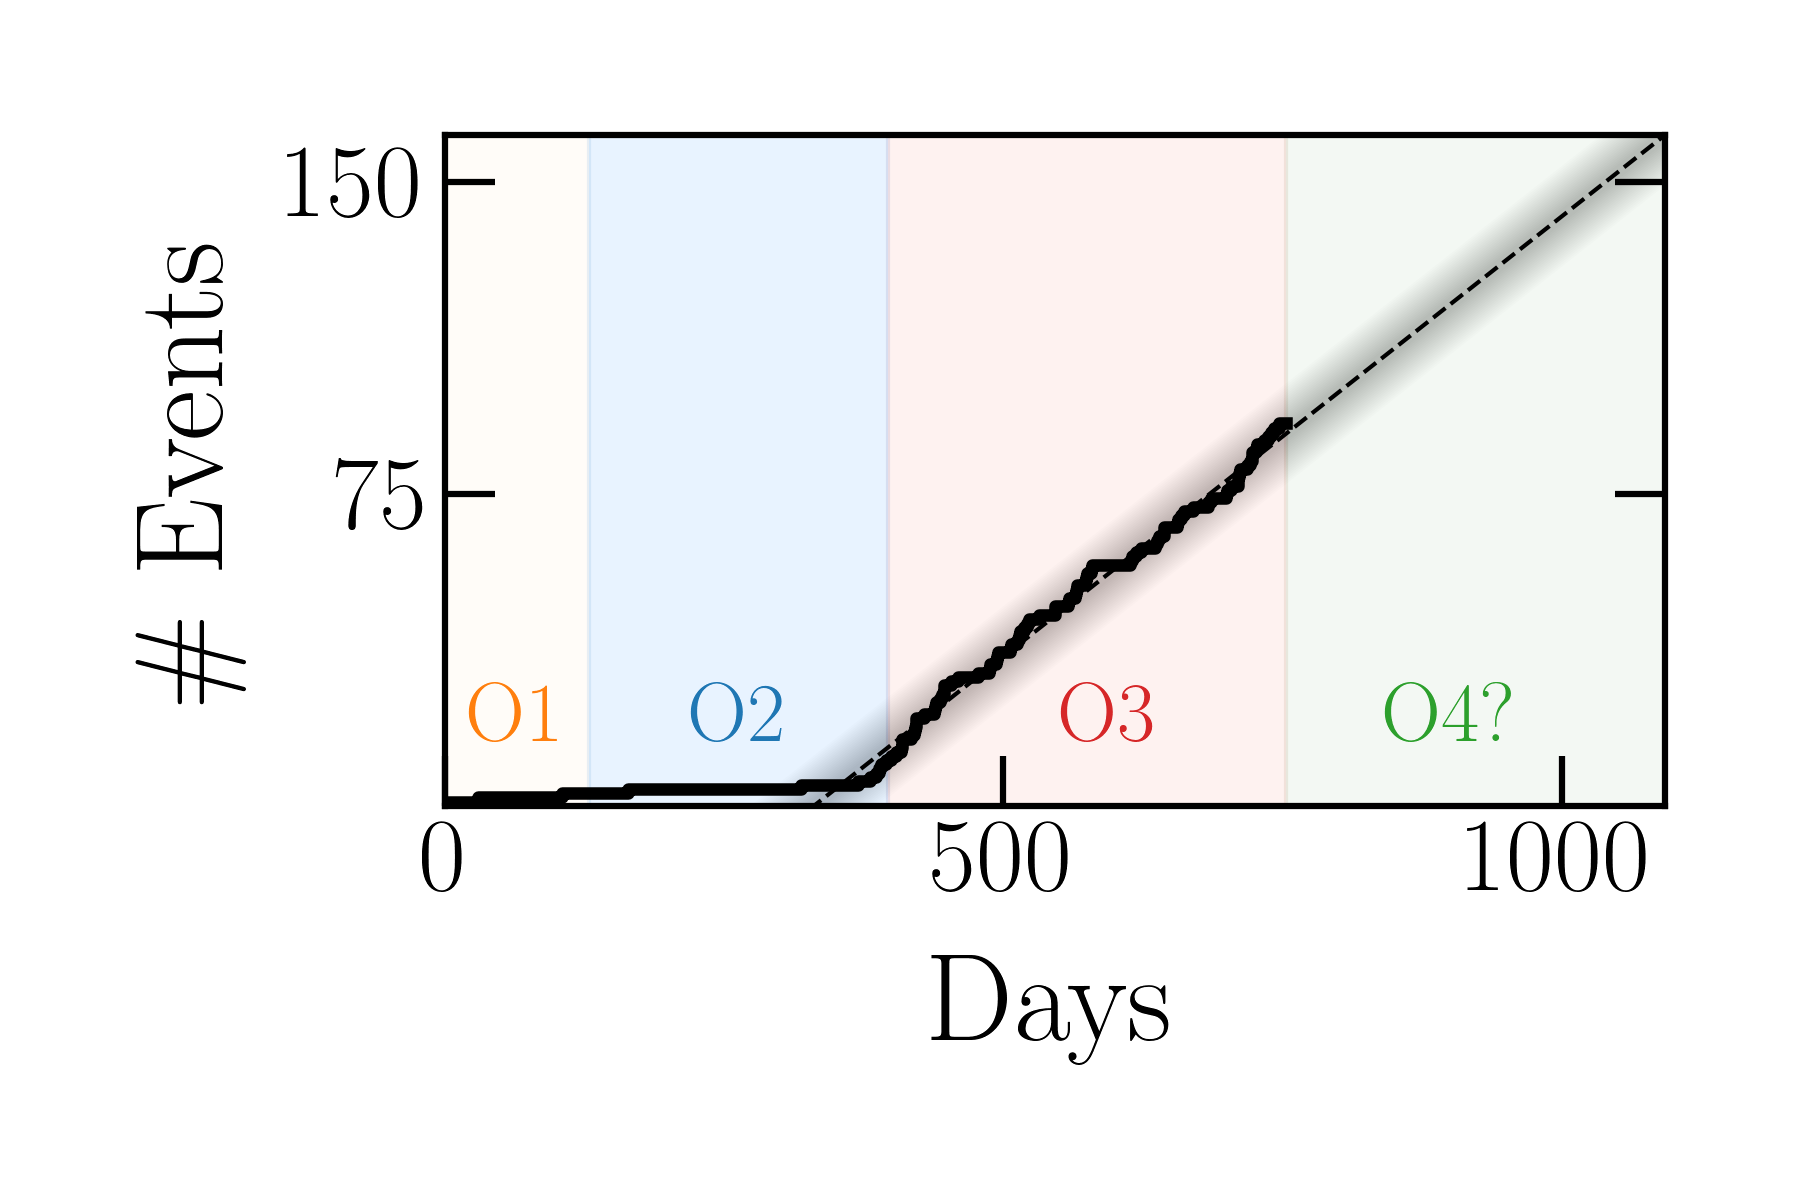
\includegraphics[width=1.\linewidth]{src/figures/gw_detection_timeframe.png}}
  \caption{\textbf{Cumulative Count of LVK Events:} The cumulative count of GW events on the vertical axis versus the number of observing days on the horizontal axis. O3 increased the count from 10 events to 93. The solid black curve is the true LVK cumulative count. The dashed black line estimates the increase in events during the fourth observing run (assuming that the O4 detection rate will be the same as O3's.  \github{https://github.com/avivajpeyi/cbc_gw_catalog_plotter}}
  \label{fig:accumulation_of_gw_events}
\end{center}
\end{figure}

The LIGO, VIRGO and KAGRA detectors have made GW astronomy a reality. 
Over the past eight years, the detections made have been a scientific goldmine. 
The detections have allowed us to study black hole mass spectrum~\cite{gwtc3_pop_inf}, test general relativity~\cite{gr_tests_gwtc3}, measure cosmological parameters~\cite{Abbott:2017:Natur, multimessenger_gw_h0, 190521_H0, Mukherjee:2022:arXiv} and probe various neutron-star equations of state~\cite{Annala:2018:PhRvL}. 
Soon, the next LVK observing run, O4, will provide astronomers with more events to study the universe. 
Figure~\ref{fig:accumulation_of_gw_events} shows the increase in GW events over the first three observing runs. 
It also provides a conservative estimate of the number of events in O4 (more detections are expected due to the detector upgrades).
However, even with the events that might be detected by the end of O4 and O5, the current GW detectors can only provide a glimpse of the full gravitational-wave universe. 

The next generation  of detectors will broaden this view. 
Plans for ground-based detectors such as CE (Cosmic Explorer~\cite{Reitze:2019:BAAS}) and ET (Einstein Telescope~\cite{Maggiore:2020:JCAP}), and even the spaced-based detector LISA (Laser Interferometer Space Antenna~\cite{Amaro-Seoane:2017:arXiv}) have been progressing in a positive direction. 
LISA will permit gravitational wave astronomers to study an entirely new spectrum of gravitational waves. 
For example, LISA will allow us to probe the merger of massive and supermassive black holes and inspirals of compact objects such as white dwarf stars and neutron stars~\cite{Amaro-Seoane:2017:arXiv}. 
The next generation ground-based detectors (XG) will probe the same gravitational wave spectrum as the current LVK detectors. 
However, the XG detectors will be over ten times more sensitive than the current detectors~\cite{Reitze:2019:BAAS, Maggiore:2020:JCAP}. 
Figure~\ref{fig:ligo_vs_ce} compares the sensitivity of CE and LIGO A+ (advanced LIGO). 
As shown in Figure~\ref{fig:ligo_vs_ce}a while the maximum distance the LIGO A+ can probe is $z\sim10$, CE can use gravitational waves to probe the edge of the observable universe at $z\sim100$~\cite{Reitze:2019:BAAS}. 
This will allow astronomers to study the black hole mass spectrum as a function of redshift, and possibly find primordial black holes~\cite{Reitze:2019:BAAS}.
\begin{figure}
\begin{center}
  \centerline{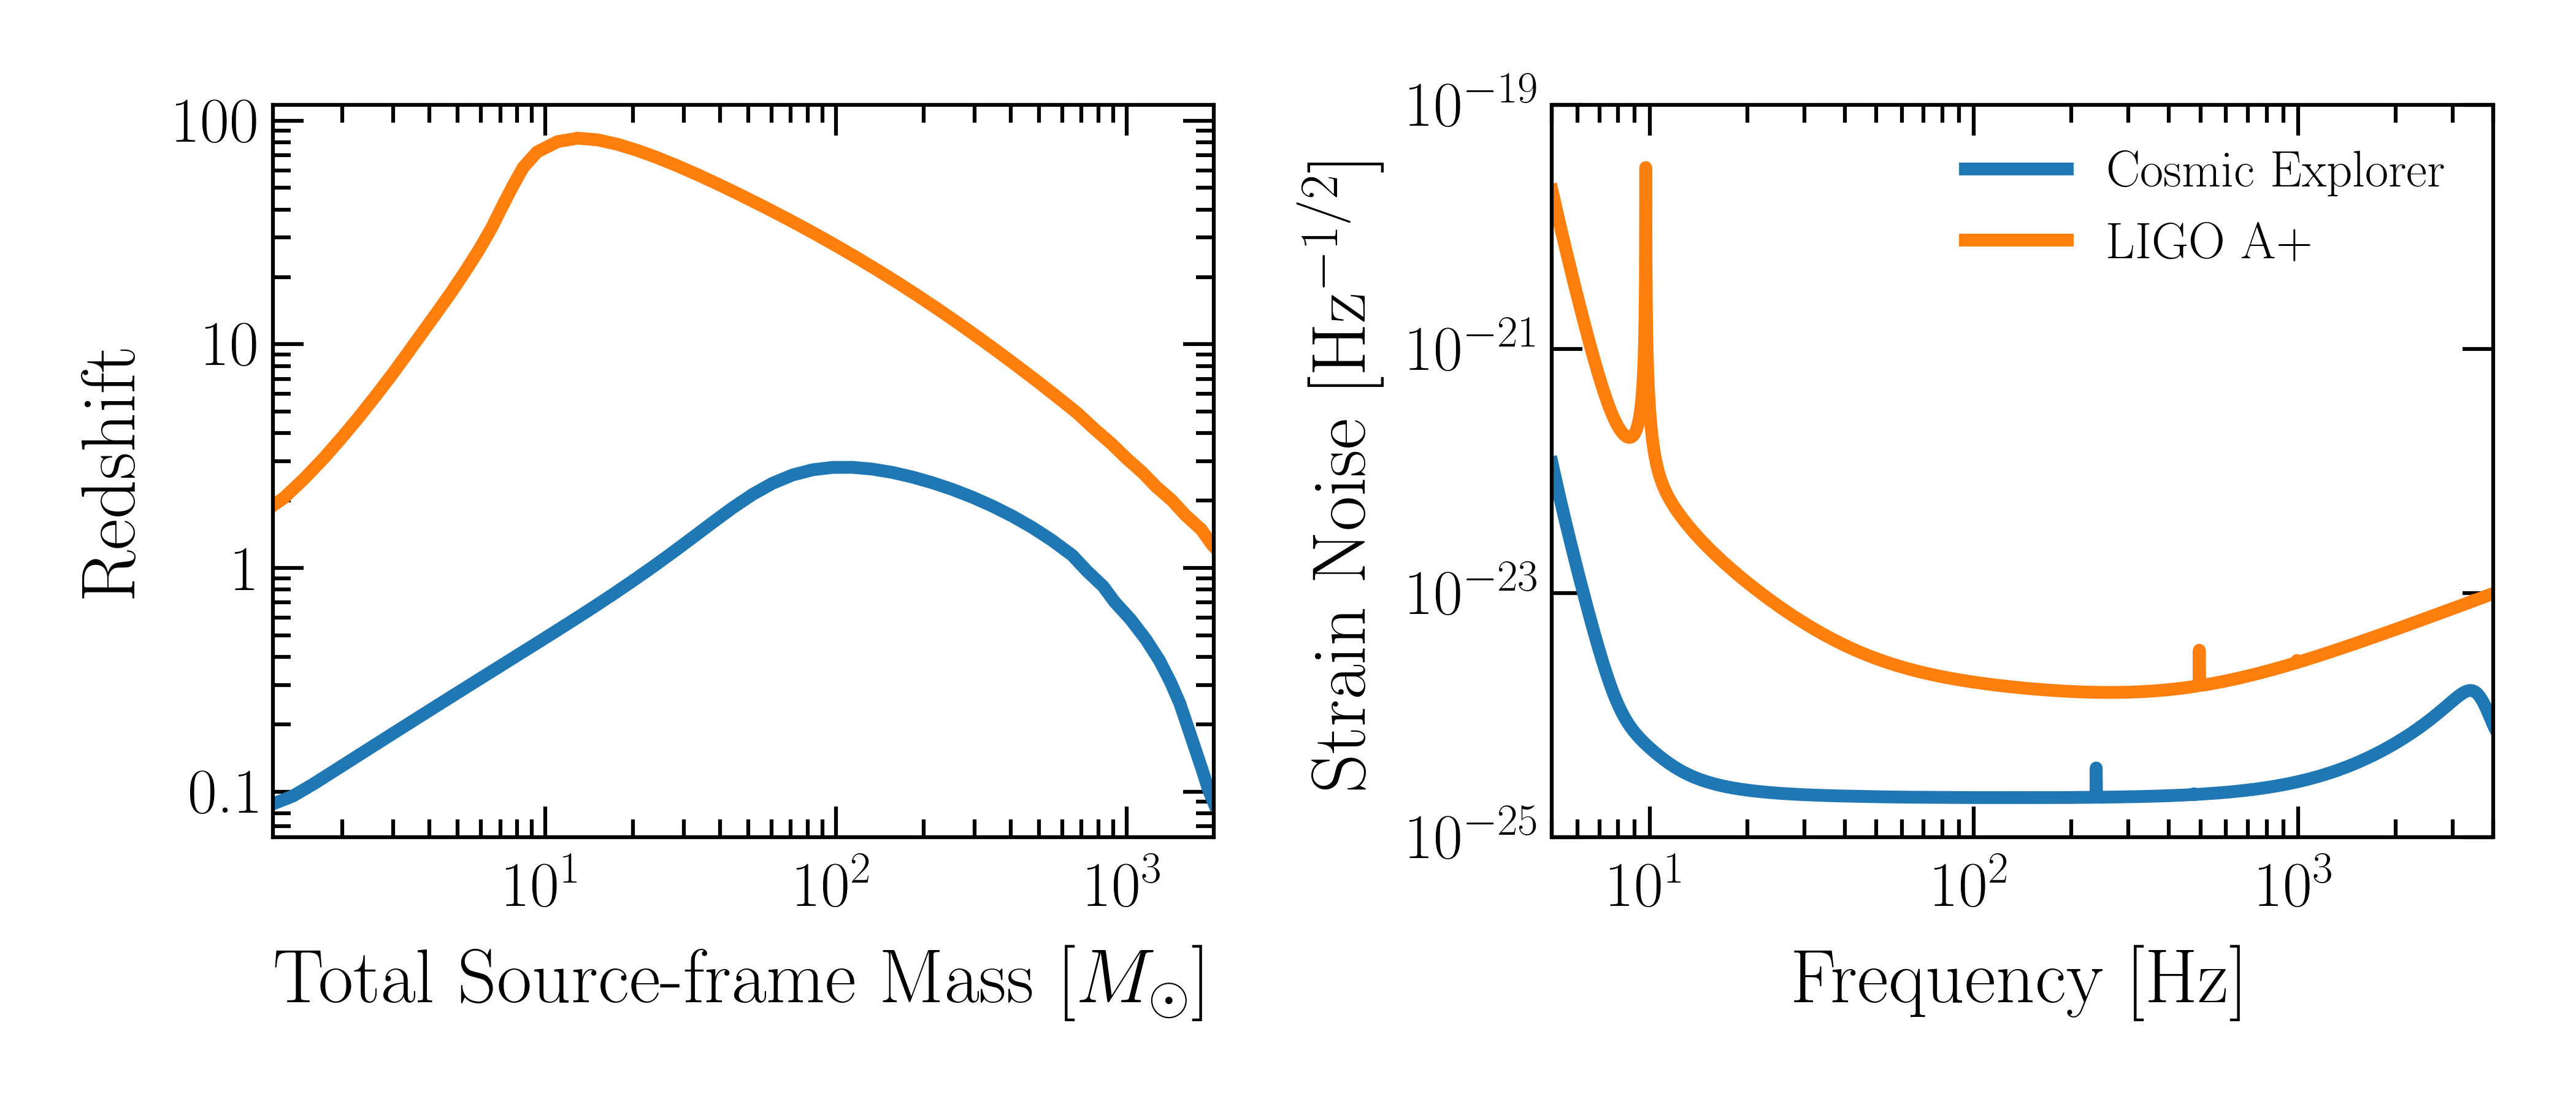
\includegraphics[width=1.\linewidth]{src/figures/ligo_vs_ce.png}}
  \caption{\textbf{LIGO A+ and CE Comparisons:}  \github{https://github.com/avivajpeyi/cbc_gw_catalog_plotter}}
  \label{fig:ligo_vs_ce}
\end{center}
\end{figure}


\textbf{Exoplanet atmospheres: the next frontier:}

Since the 1990s, an entire generation has grown up knowing that planets exist outside our solar system. Will future generations grow up knowing life exists outside our solar system?

Missions like Kepler and TESS have aided astronomers in their search to answer this question. Scientists have discovered thousands of exoplanets using data collected by these telescopes.
The exoplanet count will rise even higher with the help of future observatories like the Nancy Grace Roman Space Telescope~\cite{johnson2020predictions}.
Some confirmed exoplanets are gas giants, while others are Earth-sized, rocky planets~\cite{Stassun:2018:AJ, Guerrero:2021:ApJS}. 
Some of these planets also orbit their host star’s habitable zone~\cite{Gillon:2017:Natur, Wolf:2017:ApJL, Agol:2021:PSJ, Zechmeister:2019:AA}.
In this region, exoplanets' surface temperatures are likely to be adequate to support liquid water, a necessary condition for the emergence of life (as we know it).

However, knowing that a planet is a rocky world that orbits in the habitable zone is not enough to determine whether or not the planet hosts life.
Atmospheric conditions on exoplanets are the next research frontier~\cite{seager2010exoplanet}.
The presence of atmospheric water vapour (an indicator of water oceans) can answer if planets are possibly habitable, while the presence of biosignature gases can answer if planets are possibly inhabited~\cite{seager2010exoplanet}.

With the help of the newly launched James Webb Space Telescope (JWST), astronomers have detected carbon dioxide and water on several massive exoplanets for the first time~\cite{gardner2006james, early2022identification, pontoppidan2022jwst}.
Unfortunately, JWST lacks the power necessary to investigate atmospheres of Earth-sized exoplanets~\cite{pontoppidan2022jwst}.
ARIEL (Atmospheric Remote-sensing Infrared Exoplanet Large-survey) is a mission being developed by the European Space Agency to investigate the atmospheres of distant worlds~\cite{puig2016ariel}.
With its 2029 launch, ARIEL will analyze the chemical composition and thermal structures of hundreds of exoplanet atmospheres~\cite{puig2016ariel}.
ARIEL's observations may be the key to discovering life beyond Earth.

